%%%%%%%%%%%%%%%%%%%%%%%%%%%%%%%%%%%%%%%%%%%%%%%%%%%%%%%%%%%%%%%%%%%%%%%%%%%
%% This file is part of the book
%%
%% Algorithmic Graph Theory
%% http://code.google.com/p/graph-theory-algorithms-book/
%%
%% Copyright (C) 2009--2011 Minh Van Nguyen <nguyenminh2@gmail.com>
%%
%% See the file COPYING for copying conditions.
%%%%%%%%%%%%%%%%%%%%%%%%%%%%%%%%%%%%%%%%%%%%%%%%%%%%%%%%%%%%%%%%%%%%%%%%%%%

\documentclass{article}

\usepackage{subfigure}
\usepackage{tikz}
\usetikzlibrary{external}
\tikzexternalize{union-intersection-graphs-overlapping-vertex-sets}

\begin{document}

\begin{figure}
%% graph G_1
\subfigure[$G_1$]{
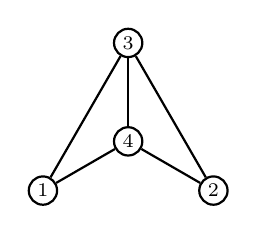
\begin{tikzpicture}
[lineDecorate/.style={-,thick},%
  nodeDecorate/.style={shape=circle,inner sep=1.5pt,draw,thick},%
  scale=1.25]
\scriptsize
%% nodes or vertices
\foreach \nodename/\x/\y in {1/-0.8660/-0.5, 2/0.8660/-0.5, 3/0/1, 4/0/0}
{
  \node (\nodename) at (\x,\y) [nodeDecorate] {$\nodename$};
}
%% edges or lines
\path
\foreach \startnode/\endnode in {1/3, 1/4, 2/3, 2/4, 3/4}
{
  (\startnode) edge[lineDecorate] node {} (\endnode)
};
\end{tikzpicture}
}
%%
%%
\quad
%% graph G_2
\subfigure[$G_2$]{
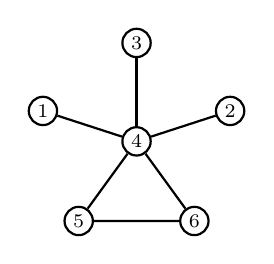
\begin{tikzpicture}
[lineDecorate/.style={-,thick},%
  nodeDecorate/.style={shape=circle,inner sep=1.5pt,draw,thick},%
  scale=1.25]
\scriptsize
%% nodes or vertices
\foreach \nodename/\x/\y in {
  1/-0.9510/0.3090, 2/0.9510/0.3090, 3/0/1, 4/0/0, 5/-0.5877/-0.8090,
  6/0.5877/-0.8090}
{
  \node (\nodename) at (\x,\y) [nodeDecorate] {$\nodename$};
}
%% edges or lines
\path
\foreach \startnode/\endnode in {1/4, 2/4, 3/4, 4/5, 4/6, 5/6}
{
  (\startnode) edge[lineDecorate] node {} (\endnode)
};
\end{tikzpicture}
}
%%
%%
\quad
%% graph G_1 union G_2
\subfigure[$G_1 \cup G_2$]{
\label{fig:introduction:union_graphs_overlapping_vertex_sets}
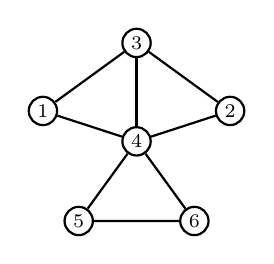
\begin{tikzpicture}
[lineDecorate/.style={-,thick},%
  nodeDecorate/.style={shape=circle,inner sep=1.5pt,draw,thick},%
  scale=1.25]
\scriptsize
%% nodes or vertices
\foreach \nodename/\x/\y in {
  1/-0.9510/0.3090, 2/0.9510/0.3090, 3/0/1, 4/0/0, 5/-0.5877/-0.8090,
  6/0.5877/-0.8090}
{
  \node (\nodename) at (\x,\y) [nodeDecorate] {$\nodename$};
}
%% edges or lines
\path
\foreach \startnode/\endnode in {1/4, 1/3, 2/3, 2/4, 3/4, 4/5, 4/6, 5/6}
{
  (\startnode) edge[lineDecorate] node {} (\endnode)
};
\end{tikzpicture}
}
%%
%%
\quad
%% graph G_1 intersect G_2
\subfigure[$G_1 \cap G_2$]{
\label{fig:introduction:intersection_graphs_overlapping_vertex_sets}
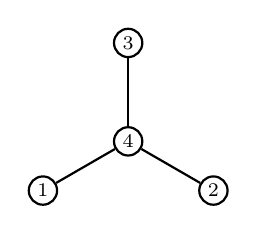
\begin{tikzpicture}
[lineDecorate/.style={-,thick},%
  nodeDecorate/.style={shape=circle,inner sep=1.5pt,draw,thick},%
  scale=1.25]
\scriptsize
%% nodes or vertices
\foreach \nodename/\x/\y in {1/-0.8660/-0.5, 2/0.8660/-0.5, 3/0/1, 4/0/0}
{
  \node (\nodename) at (\x,\y) [nodeDecorate] {$\nodename$};
}
%% edges or lines
\path
\foreach \startnode/\endnode in {1/4, 2/4, 3/4}
{
  (\startnode) edge[lineDecorate] node {} (\endnode)
};
\end{tikzpicture}
}
\end{figure}

\end{document}
